\chapter{Introdução}
A robótica costuma ser uma área bem atrativa para qualquer pessoa, seja ela conhecedora ou não do assunto. Devido a esse interesse, o ramo da robótica vem se tornando particularmente popular nos últimos anos. A robótica móvel, em especial, vem agaranhando fãs ao redor do mundo, que buscam a possibilidade de contruir seus próprios robôs e programá-los para uma função específica. Os kits de robótica ganharam espaço no mercado devido à sua completude, pois contém motores e sensores diversos e também devido ao seu baixo custo, se comparado com robôs mais avançados. Com a popularização do uso dos kits de robótica, vários torneios de robótica foram iniciados, atraindo jovens estudantes, universitários e profissionais da área. 

Esse capítulo está organizado em cinco sessões, sendo essas: Contextualização, Justificativa, Questão de Pesquisa, Objetivos e Organização dos Capítulos, todos devidamente detalhados a seguir.

\section{Contextualização}

O termo robô surgiu em meados do século XX, derivado da palavra tcheca \textit{robota}, que significa trabalhador forçado (ou escravo) \cite{da2009roboeduc}. Desde esta época, a propagação do conceito de robôs está acontecendo de forma acelerada, seja por filmes de ficção científica, ou documentários, ou desenhos animados. 
Os robôs saíram, de fato, da ficção científica em 1961, quando Joseph Engelberger desenvolveu o primeiro robô comercial, o UNIMATE e, desde então, estão cada dia mais inseridos em meio a sociedade, seja como elevadores, caixas eletrônicos, robôs de entretenimento ou de chão de fábrica \apud{murphy2000introduction}{da2009roboeduc}. 
Segundo \cite{da2009roboeduc}, um robô deve ter, idealmente, os seguintes elementos:
\begin{itemize}
\item atuadores: são os meios utilizados para que o robô se locomova e/ou altere a forma de seu corpo. Exemplo: pernas, rodas, articulações, garras, dentre outros;
\item sensores: são os meios utilizados pelo robô para medir e conhecer o ambiente, detectando objetos, calor ou luz, e convertendo essa informação em símbolos processados por computadores;
\item computador: é o responsável por controlar o robô através de algoritmos nele implementados;
\item equipamentos ou mecanismos: são ferramentas ou equipamentos mecânicos.
\end{itemize}

Um robô pode ser categorizado em um dos três grupos, atualmente conhecidos: manipuladores, móveis e híbridos. Os robôs manipuladores são fixos ao seu local de trabalho; os móveis se locomevem por meio dos atuadores, e os híbridos são um composto das duas categorias anteriores  \apud{russel2004inteligencia}{da2009roboeduc}.

A robótica é uma ciência, em rápida ascenção, que envolve áreas do conhecimento como: microeletrônica, computação, engenharia mecânica, inteligência artificial, física, neurociência, entre outras. Portanto, estuda tecnologias associadas ao projeto, fabricação, teoria e aplicação dos robôs.
	
Sendo a robótica uma área tão inter e multidisciplinar, usá-la como instrumento de aprendizagem é um tanto quanto benéfico, pois ensina à criança e/ou ao jovem a trabalhar em equipe, desenvolver o raciocínio lógico através de problemas concretos, e estimula a leitura, exploração, investigação, criatividade e organização. Além de aprimorar a parte motora do indivíduo ao trabalhar com o hardware do robô, também é aprimorado o raciocínio lógico e a abstração ao programar o software do robô \cite{da2009roboeduc}. 

Em meados dos anos 60, Seymourt Papert, reconhecido matemático, educador e pesquisador do MIT\footnote{http://web.mit.edu} (Instituto de Tecnologia de Massachusetts), criou a linguagem de programação LOGO. Essa linguagem foi utilizada nos kits educacionais da LEGO, conferindo o início do sistema educacional LEGO-LOGO. Nesse sistema, as crianças têm a possibilidade de construir seus robôs protótipos com os blocos de montagem e outros recursos do kit educacional da LEGO bem como programar com a linguagem LOGO, gerando o comportamento desejado nesses protótipos \cite{da2009roboeduc}.

Um dos kits de robótica mais populares criados pela LEGO é o Mindstorms \cite{da2009roboeduc}, que combina um computador programável, NTX ou RCX dependendo da versão, com motores elétricos, engrenagens, peças de encaixe, polias, roscas, dentre outros. Este kit contêm cerca de mil peças LEGO, incluindo o computador, o CD-ROM do software Mindstorms, um transmissor infravermelho para envio de programas para o robô (apenas para a versão RCX), um guia do construtor, motores, sensores, rodas, pneus, conectores e outros. Para aprimorar o aprendizado, a LEGO disponibiliza, além do kit de peças para montagem dos robôs, um tapete de missões a serem realizadas pelos mesmos. Cada missão do tapete tem uma pontuação máxima, que poderá ser alcançada se a missão for completada dentro do tempo e sem penalidades. É possível completar 'n' missões dentro do tempo limite.

\section{Justificativa}

Retomando aspectos apontados na contextualização, seguem algumas preocupações intrínsecas desse contexto, com as quais procura-se justificar as necessidades desta pesquisa: (i) de uma investigação mais detalhada quanto à literatura associada; (ii) da elicitação de soluções candidatas, apoiadas na Engenharia de Software, na Inteligência Artificial e no projeto e análise de algoritmos, e (iii) da implementação de uma solução dentre as elicitadas.

O curso de Engenharia de Software da UnB/FGA oferece uma disciplina chamada Princípios de Robótica Educacional. Dentre os objetivos dessa disciplina, tem-se a intenção de formar grupos de granduandos para competições em robótica nos âmbitos regional, nacional e internacional. Nesse contexto, são estabelecidos desafios aos grupos de alunos matriculados na disciplina. Esses desafios orientam-se pelas propostas de atividades da First LEGO League \cite{kamenfirst}. Uma preocupação intrínseca dos grupos participantes consiste em lidar com diferentes variáveis, em tempo de competição. No caso, destacam-se: tempo total estabelecido para conclusão das missões, localização atual do robô e pontuação das missões.

No intuito de colaborar na formação de uma equipe competitiva, têm-se como preocupações a serem investigadas nesse Trabalho de Conclusão de Curso, principalmente:

\begin{itemize}
\item O fato do tempo total para a conclusão das missões ser relativamente curto para que todas sejam realizadas, logo são necessários algoritmos que permitam a seleção dessas missões considerando o tempo como um fator impactante.

\item Seleção das missões de forma apropriada, na qual outras variáveis, além do tempo, devem ser consideradas, tais como: 
\begin{itemize}
\item Localização atual do robô, pois dependendo da posição do robô em relação ao tapete o tempo de locomoção para realizar uma missão irá mudar.   
\item Pontuação das missões, pois pode existir uma missão 'X' que gaste o mesmo tempo para ser realizada que uma missão 'Y', porém 'X' tem uma maior pontuação que 'Y', logo será mais valoroso executar a missão 'X' do que a missão 'Y'.
\end{itemize} 
\end{itemize}
 

Diante do exposto, acredita-se que a elaboração de uma base de conhecimento orientada ao Paradigma Lógico \cite{tucker2009linguagens}, especificamente implementada com base em algoritmos da Inteligência Artificial, conferirá ao robô a capacidade de gerar um roteiro de missões, sendo esse o de maior pontuação possível de ser realizada dentro do tempo restante.

Pretende-se, com tal esforço, agregar valor na formação de uma equipe competitiva em robótica, disponibilizando uma máquina de raciocínio apoiada em algoritmos avançados e instigando os membros da equipe a refinarem essa máquina de forma contínua e evolutiva, ou seja, ir aprimorando-a de acordo com as necessidades.

\section{Questão de pesquisa}

Este TCC buscará responder ao seguinte questionamento: É possível implementar inteligência artificial no robô LEGO Mindstorms, isto é uma máquina de raciocínio lógico, de tal forma que dada uma posição (X0, Y0) e um tempo restante, esse robô consiga gerar um roteiro de missões a serem executadas para alcançar a maior pontuação possível?

\section{Objetivos}
Os objetivos deste trabalho foram classificados quanto à objetivo geral e objetivos específicos, sendo ambos apresentados a seguir.

\subsection{Objetivo geral}
Desenvolver uma máquina de raciocínio lógico, considerando um algoritmo específico para tomada de decisões, com a qual o robô deverá ser capaz de selecionar as missões, compondo um roteiro, de forma que a pontuação seja maximizada em relação ao tempo disponível, previamente estabelecido.

\subsection{Objetivos específicos}
Com base no objetivo geral, foram propostos os seguintes objetivos específicos deste TCC:
\begin{itemize}
\item Investigar algoritmos candidatos à solução da questão de pesquisa considerando, em um primeiro escopo dessa atividade, o estudo de algoritmos gulosos, programação dinâmica e paradigma lógico;
\item Implementar uma solução que agregue ao robô a capacidade de gerar roteiros de missões de máxima pontuação a partir de um ponto inicial e um tempo restante.
\item Estudar o funcionamento do kit educacional LEGO Mindstorms visando a realização de uma pesquisa exploratória e experimental que permita a verificação quanto a pertinência da solução estabelecida para o contexto investigado.
\item Estabelecer uma metodologia de desenvolvimento, orientada às boas práticas da 	Engenharia de Software, no intuito de conduzir o processo investigativo, a implementação da solução bem como a verificação dessa solução no contexto acordado.
\end{itemize}

\section{Metodologia de Pesquisa}
Este trabalho é classificado quanto à natureza como pesquisa aplicada, pois tem por objetivo gerar conhecimento para a solução de um problema específico \cite{moresi2003metodologia}, o desenvolvimento de uma máquina de raciocínio para tomada de decisões estratégicas em robótica educacional.

Quanto à abordagem, esta pesquisa é classificada como qualitativa, pois a fonte direta de coleta de dados é o ambiente natural estudado, campeonatos de róbotica da Fisrt Lego League, e não requer o uso de métodos e técnicas estatísticas \cite{moresi2003metodologia}.

Quanto à tipologia, este trabalho é classificado como descritivo, pois objetiva estabelecer relações entre variáveis \cite{moresi2003metodologia}, sendo elas: tempo restante de competição, pontuação de cada missão e tempo de execução de cada missão. Essas váriáveis estão contidas em uma base de conhecimento, e a partir dela foi criado um algoritmo, baseado em programação dinâmica, que gera um roteiro de missões que devem ser executadas pelo robô, para que a maior pontuação seja atingida. 

Quanto aos procedimentos técnicos, são utilizados nesse trabalho a pesquisa bibliográfica, que tem como base livros e artigos científicos, e a experimental que será baseada em cenários de uso, cada um com o conjuto diferente de missões disponíveis para a geração do roteiro.

Quanto às técnicas de coleta de dados, neste trabalho serão utilizados a bibliografia e a observação sistemática. A Figura \ref{metodologiaPesquisa} apresenta de forma resumida essa classificação.


\FloatBarrier
\begin{figure}[!h]
\centering
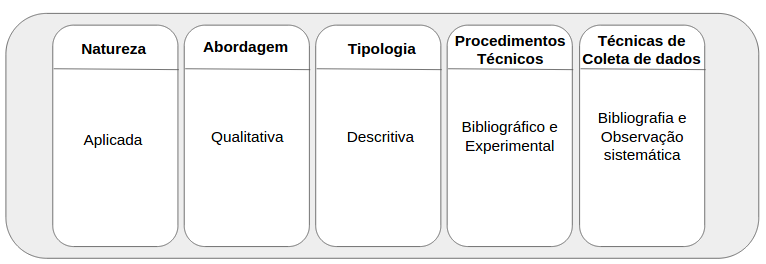
\includegraphics[keepaspectratio=true,scale=0.5]{figuras/metodologiaPesquisa.png}
\caption{Classificação da metodologia de pesquisa}
\label{metodologiaPesquisa}
\end{figure}

Segundo \citeonline{andre2008estudo} uma pesquisa é executada de acordo com três fases: Planejamento, Coleta de dados e Análise de dados.Tais fases foram adotadas por este trabalho e estão organizadas na Figura \ref{fasesPesquisa}.
\clearpage

\FloatBarrier
\begin{figure}[!h]
\centering
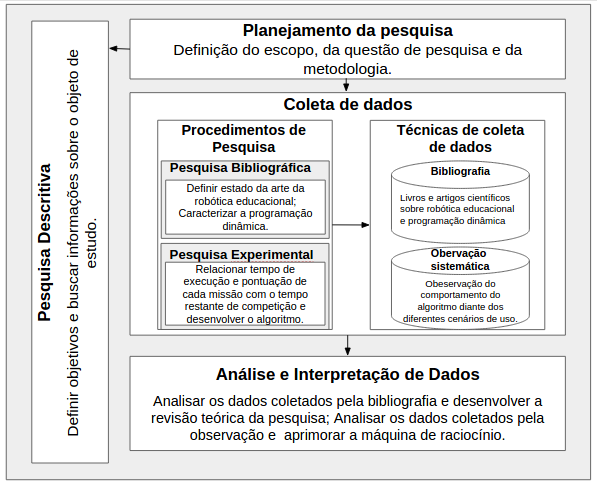
\includegraphics[keepaspectratio=true,scale=0.8]{figuras/fasesPesquisa.png}
\caption{Fases da pesquisa}
\label{fasesPesquisa}
\end{figure}

A fase de planejamento consiste em definir o objeto de estudo, o escopo do estudo, a questão de pesquisa e a metodologia de pesquisa, com os devidos procedimentos e instrumentos de coleta. Na fase de coleta de dados se aplicam os procedimentos de coleta
são aplicados. Por fim, na última fase os dados são analisados e os resultados são relatados.

Na fase de coleta de dados são utilizadas as técnicas de revisão bibliográfica e observação sistemática, detalhadas a seguir.
\begin{itemize}
\item \textbf{Revisão bibliográfica} 

Pesquisa realizada nas principais bases de dados e livros, com foco na caracterização: (i) da evolução da robótica até a sua utilização no âmbito educacional; (ii) do estado da arte da robótica móvel; (iii) dos algoritmos de otimização, como algoritmo guloso e programação dinâmica, e (iv) do paradigma lógico de programação.

\item \textbf{Observação sistemática}

Observação conduzida de acordo com um planejamento para responder ao seguinte questionamento: a máquina de raciocínio está satisfatória? Para chegar a resposta desta questão são utilizados critérios de avaliação, previamente estabelecidos.

\end{itemize}
\section{Organização dos capítulos}
Este trabalho de conclusão de curso está organizado em seis capítulos, sendo o primeiro dedicado à Introdução. Os demais são brevemente descritos a seguir:
\begin{itemize}
\item Referencial teórico: explana sobre a evolução da robótica educacional, principais conceitos do Paradigma Lógico e da programação dinâmica. 
\item Suporte tecnológico: descreve as tecnologias utilizadas no desenvolvimento
tanto da máquina de raciocínio quanto da prova de conceito, apresentando ferramentas, \textit{plugins} e \textit{kits} utilizados.
\item Materiais e métodos: aborda, dentre outros detalhes, o fluxo das atividades, detalhando como cada etapa de desenvolvimento foi executada, de acordo com o cronograma bem como os resultados obtidos em cada etapa.
\item Conclusão: efetua uma reflexão sobre o trabalho de forma a concluir se todos os objetivos estabelecidos foram atingidos e a questão de pesquisa respondida, bem como relaciona trabalhos futuros.
\end{itemize}


